\chapter{Coordinate Transformations and Alignment}
Want to align images, find their geometric relationship. If they don't align we need to perform transformations s.t. they align properly.

\section{Coordinate Transformations}

Transform image according to map $T : \mathbb{R}^2 \rightarrow \mathbb{R}^2$.

\textbf{How to generate transformed image?}

Given image $f$ in region $\Omega \subset \mathbb{R}^2$, mapping $T: \Omega \rightarrow \mathbb{R}^2$, we want to generate image $g$ in region $\Omega' \subset \mathbb{R}^2$, s.t., $g(T(\mathbf{p})) = f(\mathbf{p}), $ for all $\mathbf{p} \in \Omega$. $T$ might map outside the region...

\textbf{Naive approach (Forward Splatting):} Compute location for every pixel, throw away the pixel if it isn't in the new region and copy it to $g$ if it is.

\textbf{Problems with forward splatting:} What if $\mathbf{p'}$ not on integer pixel location?

\begin{itemize}
    \item Round coordinates, putting it to the nearest pixel - result: sever aliasing, unstable
    \item Better: Distribute among neighbors with weighting kernel
    \item Keep track of per-pixel weights, normalize
    \item Called \textbf{splatting}, suffer from aliasing and blur!
\end{itemize}

Appearance of cracks and holes, especially when magnifying..

\textbf{Implementation II: Inverse Warp}

Approach: Compute location $\mathbf{p} = T^{-1}(\mathbf{p'})$, boundary conditions apply, copy value again. Needs knowledge about the inverse map.

\textbf{Concentrate on linear maps, can be represented only with a few parameters!}

\subsection{Linear Transformations}

Map which can be written as $T(\mathbf{p}) = A\mathbf{p}$, $A \in \mathbb{R}^{2\times 2}$.

Common linear map: \textbf{Scaling} - $A = \left[\begin{matrix}s_x & 0 \\ 0  & s_y \end{matrix}\right]$, $s_x , s_y \neq 0$. \textbf{Rotation} - $A = \left[\begin{matrix}\cos \Theta & -\sin \Theta \\ \sin \Theta  & \cos \Theta \end{matrix}\right]$

Compositions of $n$ linear maps $T_1, \dots, T_n$ can be written as concatenation of application in the right order $T_n(\dots(T_1(\mathbf{p})\dots ) = A_n A_{n-1} \dots A_1 \mathbf{p} = A \mathbf{p}$. Composition of linear maps is linear, duh.

\textbf{SVD:} Can get all information about linear maps by looking at \textbf{SVD}. $A = U \Sigma V^T$, we know $A$ maps $V$ onto scaled $U$. Another interpretation: Linear trans. can be written as \textbf{rotation} $V^T$ followed by scaling $\Sigma$, followed by another \textbf{rotation} $U$.

\textbf{Properties:} \textit{Origin maps to origin, Lines map to lines, parallel lines remain parallel, ratios are preserved, closed under composition}!

\subsection{Affine Transformations}
Translation missing in linear trans. Hence, we generalize to \textbf{affine} transformation, applying linear trans. $A$ and afterwards translation $\mathbf{t}$, i.e., $T(x) = Ax + \mathbf{t}$.

\textbf{Properties:} \textit{Origin is not mapping to origin}, \textbf{otherwise same as linear}.

\textbf{Special cases of  Affine Transformations:} (Important, hence memorize these)

\begin{itemize}
    \item \textbf{Translation} - $A = I_2$, two degs. of freedom. I.e. only $\mathbf{t}$ changes the image.
    \item \textbf{Euclidean (rigid motion)} - $A$ pure rotation, three degrees of freedom (from translation we have two and one from rotation, i.e., the angle $\phi$)
    \item \textbf{Similarity} - $A = sR$, $R$ rotation and $s > 0$ scaling. Three DoFs from before + 1 from scaling, i.e., \textbf{4 DoF!}
    \item \textbf{Area Preserving} - $det(A)  = 1$, areas stay the same, \textbf{5 DoF!}
\end{itemize}

\subsection{Corresponding matrix groups}

Group of all invertible matrices is \textbf{general linear group}: $GL(2) = \{A \in \mathbb{R}^{2\times 2} : det(A) \neq 0\}$, operation is matrix multiplication (concatenating maps).

Subgroup of \textbf{area preserving maps}:  $SL(2) = \{A \in \mathbb{R}^{2\times 2} : det(A) = 1\}$

\textbf{Pure rotation} is  $SO(2) = \{A \in \mathbb{R}^{2\times 2} : det(A) = 1 \wedge A^T A = AA^T = 1\}$, which is a subgroup of the \textbf{orthogonal group} (allows reflection): $O(2) = \{A \in \mathbb{R}^{2\times 2} : A^T A = AA^T = 1\}$

\subsection{Moving to homogenous coordinates}

Make coordinates \textbf{homogenous} by adding a coordinate. Points on line $[wx \ wy \ w]^T$ are identified, equality holds by scaling factor $w$.

Affine maps: $T(\mathbf{p}) = A \mathbf{p} + \mathbf{t}$, Homogenous: $\widehat{T(\mathbf{p})} = \left[\begin{matrix}
    A & \mathbf{t} \\
    0 & 1
\end{matrix}\right]\left[\begin{matrix}
    \mathbf{p}\\
    1
\end{matrix}\right]$

\textbf{Two new parameters}: $H = \left[\begin{matrix}
    A & \mathbf{t} \\
    b^T & 1
\end{matrix}\right]$, i.e., $b$ which is a two row vector. The map is called homography (projective transformation or planar perspective map).

\subsection{Understanding geometry of homographies}

\textbf{Special case:} $H = \left[\begin{matrix}
1 & 0 & 0 \\ 0 & 1 & 0 \\ -\frac{1}{f} & 0 & 1 
\end{matrix}\right]$, with $f \neq 0$. Then applied to a point, the image of $[x \ y]^T$ is $\left[ \begin{matrix}x \\ y \\ -\frac{x}{f+1}\end{matrix} \right] \approx
\left[ \begin{matrix}\frac{fx}{f-x} \\ \frac{fy}{f-x}\end{matrix} \right]$, if $x = f$, denominator $= 0$ hence point at infinity.

\textbf{How about lines parallel to the y-axis?:} $H$ the same, let $t \in \mathbb{R}$ and $x_0$ constant, then for $[x_0 \ t \ 1]^T$, mapping is $\left[ \begin{matrix}\frac{fx_0}{f-x_0} \\ \frac{ft}{f-x_0}\end{matrix} \right]$, so we get again vertical lines. But the x-coord. changes non linearly, i.e. the distances between two vertical lines may differ!

\textbf{Horizontal lines:} $H$ again, $[t \ y_0 \ 1 ]^T, t \in \mathbb{R}$, we get $\left[ \begin{matrix}\frac{ft}{f-t} \\ \frac{fy_0}{f-t}\end{matrix} \right]$, with $t \rightarrow \infty$, we get $[-f \ 0]^T$, a point at infinity in x-direction (vanishing point).

\textbf{Special case: Two vanishing points}

$H = \left[\begin{matrix}
1 & 0 & 0 \\ 0 & 1 & 0 \\ -\frac{1}{f_x} & -\frac{1}{f_y} & 1 
\end{matrix}\right], f \neq 0, f_x = f_y = 2000$, vertical lines are now not vertical but intersect a vanishing point as  well, since we get for a point $\left[\begin{matrix}
-\frac{f_x f_y x}{f_y x + f_x y - f_x f_y} \\ -\frac{f_x f_y y}{f_y x + f_x y - f_x f_y}
\end{matrix}\right]$.

\textbf{Special case: Moving image before hand}

$H = \left[\begin{matrix}
1 & 0 & t_1 \\ 0 & 1 & t_2 \\ -\frac{1}{f_x} & 0 & 1 
\end{matrix}\right], f \neq 0$ for a point we get $\left[\begin{matrix}
-\frac{fx + ft_1}{f - x} \\ -\frac{fy + ft_2}{f-x}
\end{matrix}\right]$

\subsection{Overview and summary of coordinate transforms}

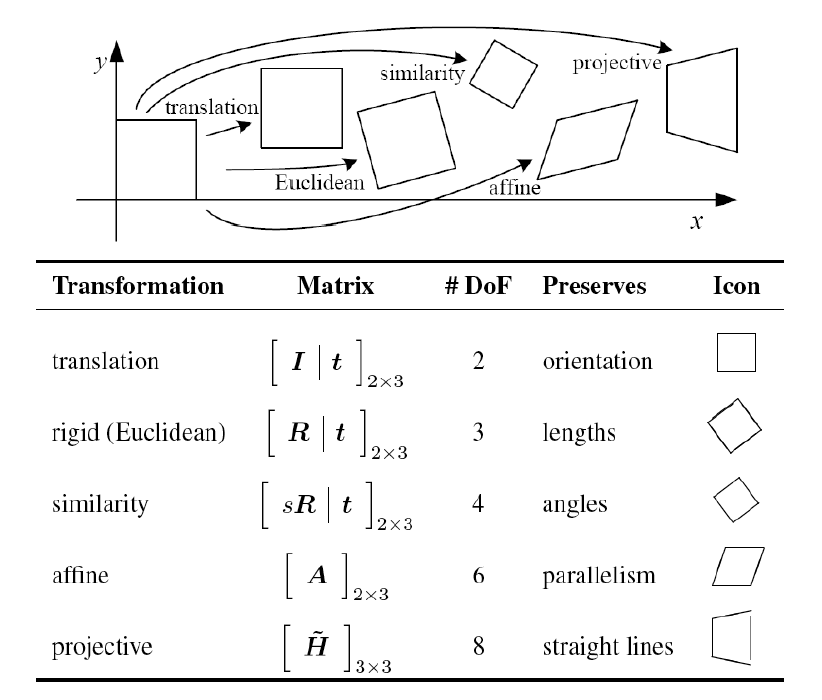
\includegraphics[width=\textwidth]{images/chap5/summ_coord_trans}

\section{Model Fitting I: Least Squares}

From now on, we want to estimate homographies using \textbf{correspondance information}

\textbf{Homography} between two image planes $\Omega, \Omega', \mathbf{p}_i \in Omega, \mathbf{p}'_i \in \Omega', 1 \leq i \leq m$, estimating $H =  \left[\begin{matrix}
h_{11} & h_{12} & h_{13} \\
h_{21} & h_{22} & h_{23} \\
h_{31} & h_{32} & 1 \\
\end{matrix}\right]$, giving us \textbf{8 Degrees of Freedom}.

\textbf{Problem:} $H$ defined in proj. coords, which is only correct up to scaling factor!

\textbf{Two equations from one coorespondance:} $\mathbf{p}_i = [x_i \ y_i \ 1]^T$ normalized, $\mathbf{p}'_i = [x'_i \ y'_i \ w'_i]$ not normalized! Then we get a linear system \begin{align*}
    x'_i & = h_{11} x_i + h_{12} y_i + h_{13} \\
    y'_i & = h_{21} x_i + h_{22} y_i + h_{23} \\
    w'_i & = h_{31} x_i + h_{32} y_i + 1
\end{align*}, from which we get the following two equations: \begin{align*}
    \frac{x'_i}{w'_i} (h_{31} x_i + h_{32} y_i + 1) - h_{11} x_i - h_{12} y_i - h_{13} & = 0 \\
    \frac{y'_i}{w'_i} (h_{31} x_i + h_{32} y_i + 1) - h_{21} x_i - h_{22} y_i - h_{23}
\end{align*}, i.e., we divide by $w'_i$ and intersect with $0$.

\begin{itemize}
    \item Correspondance leads to two equations
    \item \textbf{Problem:} Overfitting/Overdetermining by having more equations than variables
    \item 2 times correspondences equations for $8$ unknowns..
    \item Frequent problem in science!
\end{itemize}

The corresponding linear system (by correspondences) is:

$\left[\begin{matrix}
& & & & \vdots & & & \\
-x_i & -y_i & -1 & 0 & 0 & 0 & \frac{x'_i}{w'_i}x_i & \frac{x'_i}{w'_i} y_i \\
0 & 0 & 0 & -x_i & -y_i & -1 & \frac{y'_i}{w'_i}x_i & \frac{y'_i}{w'_i} y_i \\
& & & & \vdots & & &
\end{matrix}\right]\left[
\begin{matrix}
h_{11} \\h_{12} \\h_{13} \\h_{21} \\h_{22} \\h_{23} \\h_{31} \\h_{32}
\end{matrix}\right] = \left[
\begin{matrix}
\vdots \\ -\frac{x'_i}{w'_i} \\ -\frac{y'_i}{w'_i} \\ \vdots
\end{matrix}\right]
$

\textbf{Considerations}: We have $Ax = b$, looking for $x \in \mathbb{R}^n$ and $ m > n$, we often do not have an exact solution! But we can try to find \textbf{the best fit}.

\textbf{Least Squares:} Minimize distance to $b$ finding $\hat{y} = A\hat{x}$ with $\hat{x} = \mathrm{argmin}_{x\in \mathbb{R}^n} \frac{1}{2} ||Ax - b||^2$. The line from $\hat{y}$ to $b$ is orthogonal to our model, hence lowest distance. In formulas we can get the \textbf{normal equations}: $$A^T (A\hat{x} -b ) = 0 \leftrightarrow A^T A\hat{x} = A^T b$$.

\textbf{Analytic point of view:} Minimizer for $E(x) = \frac{1}{2}||Ax - b||^2$, can use the gradient which is $\nabla E(x) = A^T (Ax - b)$, i.e. the same as the geometric solution.

\textbf{Solution to the normal equations:} (\textbf{if $A^T A$ has an inverse..}) Use $SVD$, i.e. $A = U\Sigma V^T$ which reduces \textbf{normal equations} to $$\Sigma^2 V^T \hat{x} = \Sigma U^T b$$. 

With left-inverse of $\Sigma$, $\Sigma^2$ vanishes, it can be found inverting every singular value, i.e. $\Sigma^+ = \mathrm{diag}(\sigma_1^{-1}, \dots, \sigma_k^{-1}, 0 , \dots , 0)$, so we get $\Sigma^+ \Sigma = I$, with $\hat{x} = V \Sigma^+ U^T b$ and $A^+ = V \Sigma^+ U^T$ being the \textbf{pseudo inverse} of $A$!

\textbf{Weighted least squares:} Add weights $\sqrt{w_i}$ to the correspondences. Solution is same as before..

\textbf{Problems:} \begin{itemize}
    \item outliers make for bad results
    \item one strong outlier may destroy the whole result
\end{itemize}

\section{Model Fitting II: RANSAC}

\textbf{RANdom SAmple Consensus:} \begin{itemize}
    \item {Repeat $N$ times
    \begin{itemize}
        \item Select random subset of samples
        \item Compute model
        \item Compute error between samples and model
        \item Count \textbf{inliers} by using \textbf{fixed threshold}
    \end{itemize}        
    }
    \item Refit model using largest inlier set found during the $N$ iterations
\end{itemize}

\textbf{Parameters:} 

\textbf{1: Number of points selected for model fitting:} Choose minimum, since
\begin{itemize}
    \item Faster fits, more iterations in same amount of time
    \item More likely to randomly select only inliers
    \item \textbf{Tradeoff:} Initialization may not be good for minimal sample size
\end{itemize}

\textbf{2: Threshold:} Choose with 95\% probability for an inlier to stay below threshold. \textbf{Example:} Gaussian noise with $\sigma$ expected on data, 95\% of inliers will be within $2\sigma$, 99\% within $3\sigma$.

\textbf{3: Number $N$ of hypothesis trials:} 

Choose $N$ with $p$ so that one random sample is free from outliers. Given \textbf{percentage of outliers in the data $e$} we have \begin{align*}
    (1- (1-e)^s)^N & = 1 - p \\ N & = \frac{\log(1-p)}{\log(1-(1-e)^s)}
\end{align*}

The higher $s$ is chosen, the faster the number $N$ grows in relation to the outlier amount in percent. \textbf{Works well for ratios less than 50\%}!

\textbf{Problem:} $e$ unknown, hence we need adaptive approach: Start with $count = 0, e= 1$ and as long as $N > count$ \begin{itemize}
    \item Perform RANSAC as usual
    \item $e \leftarrow \mathrm{min} (e , 1 - \frac{numInliers}{numPoints})$
    \item $N \leftarrow \frac{\log(1-p)}{\log(1-(1-e)^s)}$
    \item $count \leftarrow count + 1$
\end{itemize} , i.e., we update $e$ if we find a better value of $e$ out of the inliers and point amount we look at, then $N$ can be updated.

\textbf{RANSAC on Homography estimation:}

Correspondences agree what $H$ looks like, small outlier amount does not agree.

Approach: \begin{itemize}
    \item Define max number of iterations, otherwise same as adaptive approach
    \item \textbf{In each iteration}: Select 4 correspondences randomly
    \item Compute $H$
    \item Compute error $\epsilon$ for $H$ and correspondences
    \item If the new inliers are more than previously replace everything (also $e$ and $N$ according to adaptive approach)
\end{itemize}

\textbf{PROs and CONs:}
\begin{itemize}
    \item[+] Simple/general
    \item[+] Many applications 
    \item[+] Works well in practice
    \item[-] Several parameters
    \item[-] Not deterministic
    \item[-] Iterative with unknown number $N$
    \item[-] Bad for low inlier ratios
    \item[-] Not always good initialization based on minimum number of samples
\end{itemize}

\textbf{RANSAC} is classic example for \textbf{Voting Scheme}, like \textbf{Hough transform}

\section{Model Fitting III: Hough Transform}

Just a rough look at hough transform..

\begin{itemize}
    \item \textbf{Voting Scheme} for fitting low-parameter models
    \item Detect \textbf{simple} geometric objects, represented by \textbf{very few} parameters (lines,circles)
    \item Assumptions: {\begin{itemize}
        \item Boundaries with large $|\nabla|$
        \item Points satisfy $g(\mathbf{p}, \alpha_1, \dots, \alpha_m) = 0$, $\alpha$ parameters to be determined
    \end{itemize}}
    \item \textbf{Examples:} {\begin{itemize}
        \item Line with normal $\mathbf{n} = (\cos \phi, \sin \phi)$, distance $d$ to origin can be represented as $x\cos \phi + y\sin \phi - d = 0$
        \item Circle with center $(a,b)$ radius $r$ as $|x-a| + |y-b| - r$ = 0
    \end{itemize}}
    \item \textbf{Object rep:} {\begin{itemize}
        \item Work on space of parameters
        \item Points in param space describe different objects in image space
    \end{itemize}}
    \item \textbf{Voting Strategy:} {\begin{itemize}
        \item Detect all edges
        \item Every edge point votes for all params to satisfy the upper equation
        \item Majority rule: parameters of most relevant object gets the mos votes
    \end{itemize}}
    \item \textbf{Advantages:} {\begin{itemize}
        \item No fully connected contours needed
        \item Detects all objects which fit the model
        \item Very robust
    \end{itemize}}
    \item \textbf{Disadvantages:} {\begin{itemize}
        \item Memory requirements and computational effort increases rapidly with parameters
        \item Bad parallelization..
    \end{itemize}}
\end{itemize}

\section{Summary}